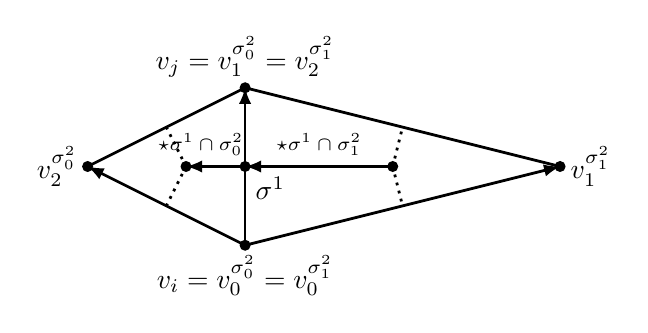
\begin{tikzpicture}[>=latex, line width=1pt]
\coordinate (Vi) at (0,-1);
\coordinate (Vj) at (0,1);
\coordinate (V02) at (-2,0);
\coordinate (V11) at (4,0);

\fill (Vi) circle (2pt) node[below] {\(v_i = v^{\sigma^2_0}_0 = v^{\sigma^2_1}_0\)};
\fill (Vj) circle (2pt) node[above] {\(v_j = v^{\sigma^2_0}_1 = v^{\sigma^2_1}_2\)} ;
\fill (V11) circle (2pt) node[right] {\( v^{\sigma^2_1}_1\)};
\fill (V02) circle (2pt) node[left] {\( v^{\sigma^2_0}_2\)};

\draw[->] (Vi) -- (Vj);
\draw[->] (Vi) -- (V11);
\draw[->] (Vi) -- (V02);
\draw (Vj) -- (V02);
\draw (Vj) -- (V11);

\coordinate (C) at (0,0);
\coordinate (C0) at (-0.75,0);
\coordinate (C1) at (1.875,0);

\fill (C) circle (2pt) node[below right] {\(\sigma^1\)};
\fill (C0) circle (2pt);
\fill (C1) circle (2pt);

\draw[->] (C1) -- node[above] {\scriptsize\(\star\sigma^1\cap\sigma^2_1\)}(C);
\draw[->] (C) -- node[above] {\scriptsize\(\star\sigma^1\cap\sigma^2_0\ \ \ \ \)}(C0);

\draw[style=dotted] (C0) -- (-1,0.5);
\draw[style=dotted] (C0) -- (-1,-0.5);
\draw[style=dotted] (C1) -- (2,0.5);
\draw[style=dotted] (C1) -- (2,-0.5);
\end{tikzpicture}